\documentclass[a4paper,12pt]{article}
\usepackage[utf8]{inputenc}
\usepackage[a4paper,
            bindingoffset=0.2in,
            left=1in,
            right=1in,
            top=1in,
            bottom=1in,
            footskip=.25in]{geometry}

%###############################################################################

%\input{~/layout/global_layout}


%###############################################################################

% packages begin

\usepackage[
  backend=biber,
  sortcites=true,
  style=alphabetic,
  eprint=true,
  backref=true
]{biblatex}
\addbibresource{bibliographie.bib}
\usepackage[acronym]{glossaries}

\usepackage{euscript}[mathcal]
% e.g. \mathcal{A} for fancy letters in mathmode
\usepackage{amsmath,amssymb,amstext,amsthm}

\usepackage{mdframed}
\newmdtheoremenv[nobreak=true]{problem}{Problem}[subsection]
\newmdtheoremenv[nobreak=true]{claim}{Claim}[subsection]
\newtheorem{definition}{Definition}[subsection]
\newtheorem{lemma}{Lemma}[claim]
\newtheorem{plemma}{Lemma}[problem]

\usepackage{mathtools}
\DeclarePairedDelimiter\ceil{\lceil}{\rceil}
\DeclarePairedDelimiter\floor{\lfloor}{\rfloor}

\usepackage{enumerate}
\usepackage[pdftex]{graphicx}
\usepackage{subcaption}
% 'draft' für schnelleres rendern mitübergeben -> [pdftex, draft]
% dadruch wird nicht das bild mitgerendered, sondern nur ein kasten mit bildname -> schont ressourcen

\usepackage{hyperref}

\usepackage{tikz}
\usetikzlibrary{arrows,automata,matrix,positioning,shapes}

% for adding non-formatted text to include source-code
\usepackage{listings}
\lstset{language=Python,basicstyle=\footnotesize}
% z.B.:
% \lstinputlisting{source_filename.py}
% \lstinputlisting[lanugage=Python, firstline=37, lastline=45]{source_filename.py}
%
% oder
%
% \begin{lstlisting}[frame=single]
% CODE HERE
%\end{lstlisting}
\usepackage{algorithm}
\usepackage{algpseudocode}

\usepackage{wasysym}

\usepackage{titling}
\usepackage{titlesec}
\usepackage[nocheck]{fancyhdr}
\usepackage{lastpage}

\usepackage{kantlipsum}
\usepackage[colorinlistoftodos,prependcaption,textsize=tiny]{todonotes}

% packages end
%###############################################################################

\pretitle{% add some rules
  \begin{center}
    \LARGE\bfseries
} %, make the fonts bigger, make the title (only) bold
\posttitle{%
  \end{center}%
  %\vskip .75em plus .25em minus .25em% increase the vertical spacing a bit, make this particular glue stretchier
}
\predate{%
  \begin{center}
    \normalsize
}
\postdate{%
  \end{center}%
}

\titleformat*{\section}{\Large\bfseries}
\titleformat*{\subsection}{\large\bfseries}
\titleformat*{\subsubsection}{\normalsize\bfseries}

\titleformat*{\paragraph}{\Large\bfseries}
\titleformat*{\subparagraph}{\large\bfseries}

%###############################################################################
% TODO define Headers and Fotter

\pagestyle{fancy}
\fancyhf{}
% l=left, c=center, r=right; e=even_pagenumber, o=odd_pagenumber; h=header, f=footer
% example: [lh] -> left header, [lof,ref] -> fotter left when odd, right when even
%\fancyhf[lh]{}
%\fancyhf[ch]{}
%\fancyhf[rh]{}
%\fancyhf[lf]{}
\fancyhf[cf]{\footnotesize Page \thepage\ of \pageref*{LastPage}}
%\fancyhf[rf]{}
\renewcommand{\headrule}{} % removes horizontal header line

% Fotter options for first page

\fancypagestyle{firstpagestyle}{
  \renewcommand{\thedate}{\textmd{}} % removes horizontal header line
  \fancyhf{}
  \fancyhf[lh]{\ttfamily M.Sc. Computer Science\\KTH Royal Institute of Technology}
  \fancyhf[rh]{\ttfamily Period 3\\\today}
  \fancyfoot[C]{\footnotesize Page \thepage\ of \pageref*{LastPage}}
  \renewcommand{\headrule}{} % removes horizontal header line
}
%###############################################################################
% Todo: define Title

\title{
  \normalsize{DD2358 VT25 Introduction to}\\
  \normalsize{High Performance Computing}\\
  \large{Project Report}
}
\author{
  \small Rishi Vijayvargiya\\[-0.75ex]
%  \footnotesize\texttt{MN: }\\[-1ex]
  \scriptsize\texttt{rishiv@kth.se}
  \and
  \small Paul Mayer\\[-0.75ex]
%  \footnotesize\texttt{MN: }\\[-1ex]
  \scriptsize\texttt{pmayer@kth.se}
}
\date{}

%###############################################################################
% define Commands

\newcommand{\N}{\mathbb{N}}
\newcommand{\R}{\mathbb{R}}
\newcommand{\Z}{\mathbb{Z}}
\newcommand{\I}{\mathbb{I}}

\newcommand{\E}{\mathbb{E}}
\newcommand{\Prob}{\mathbb{P}}

\renewcommand{\epsilon}{\varepsilon}

% Todo: Set Counter to Excercise Sheet Number
%\setcounter{section}{1}
%\setcounter{subsection}{1}

%###############################################################################
%###############################################################################

\begin{document}
\maketitle
\thispagestyle{firstpagestyle}

% \tableofcontents
\listoftodos

\vspace{1em}

% content begin
%

\section*{Prefix}
The original code for this project is taken from the following \href{https://github.com/pmocz/finitevolume-python/blob/master/finitevolume.py}{GitHub repository}.\\
The code is written by \href{https://pmocz.github.io}{Philip Mocz}.
We made following changes before starting with the project:

\begin{enumerate}
  \item Fixed a bug that resulted in an infinite loop when setting the \verb|plotRealTime| flag to \verb|False|.
  \item ...\todo{Add more bugs that may come up!}
\end{enumerate}

\tableofcontents
\newpage
\section{Introduction}
The Kelvin-Helmholz-Inequality is a phenomenom that arises when two fluid layers of different velocities interface with each other.
It results in characteristic patterns that can be observered, e.g. in clouds, the surface of the sun or in jupyters colorful atmosphere.
Philip Mocz created an which produces a visualization of the characteristic swirls of the K-H-inequality.

The Finite Volume method is a popular simulation technique to simulate fluids or partial differential equations that can be represented in a conservative form.
This is often the case for equations that describe physical conservation laws.
The Euler-Fluid-Equations (a simplifications of the Navier-Stokes-Equations) can be represented nebsts it's primitive description in such conservative form.
Within the algorithm, Philip Mosz makes use of both representations of the formula.
He uses the primitive form to extrapolate values in time and space, but uses the conservative representation to derive the update formula.
In some sorts, this gives us the best of both worlds.
Extrapolating within the primitive form is numerically more stable whereas the conservative representation is used to compute the update efficiently.
\todo{describe finite volume approach, maybe small image}
\todo{loose a word or two about boundary conditions and initial values}

The algorithm in principle works as follows:
For each timestep and each cell do
\begin{enumerate}
  \item Get cell central primitive variables (convert from conservative ones)
  \item Calculate timestep (What does that mean exactly)
  \item Calculate gradient of primitive vars (e.g using central differences)
  \item Extrapolate prim. vars. in time ($\Delta t / 2$)
  \item Extrapolate prim. vars. to faces ($\Delta x / 2$)
  \item Compute Fluxes along each face
  \item Update solution by adding Fluxes to conserv. vars
\end{enumerate}

Update Formula:
\begin{equation}
Q^{(n+1)} = Q^{(n)} - \Delta t \Delta x \sum_{j} \hat{F}_{ij}^{(n + \frac{1}{2})}
\end{equation}

We aim to introduce some optimization techniques that decrease the overall runtime of the computation.
To achieve this, we use techniques obtained from the lectures, specifically using cython to use precompiled c code to reduce python overhead,
introducing gpu accellerators using pytorch and investigate a distributed computation approach utilizing dask.

\section{Baseline tests}

\subsection{Runtime}
We approached this problem by trying to get a basic understanding of what might be the runtime bottleneck.
For this we used the line profiler.
We simulated on a 256x256 grid for 3749 iterations, which the script needs to perform a 2s simulation.
We came to the conclusion that a large portion (nearly 50\% for a single iteration) of computation time is spent to compute the fluxes (\verb|getFlux| method).
\begin{lstlisting}[language=bash,basicstyle=\scriptsize\ttfamily]
Line #      Hits         Time  Per Hit   % Time  Line Contents
==============================================================
   195                                           @profile
   196                                           def main():
[...]
   270                                                   # compute fluxes
   271      3694    5113424.0   1384.3     24.9          [...] = getFlux(...)
   272      3694    4595361.0   1244.0     22.4          [...] = getFlux(...)
[...]
\end{lstlisting}
All other function calls accumulated to the other 50\%, however each in itself were rather neglegtable (at most below 4\%).
This indicated to us that we should focus our efforts onto this part of the computation.

\subsection{Memory}
\todo[inline]{Write everything...}

\subsection{Hyperparameters\todo{This is a working title. Is there a better headline titel for this?}}
The runtime of the simulation depends on multiple parameters.
First and foremost the number of iterations:
this regulates the total time (number of time steps) we want to simulate.
Figure \ref{fig:runtime_per_iteration} displays the runtime the computation of each timestep needs.
We can observe that the runtime per iteration is mostly consistant.
\begin{figure}[h]
  \centering
  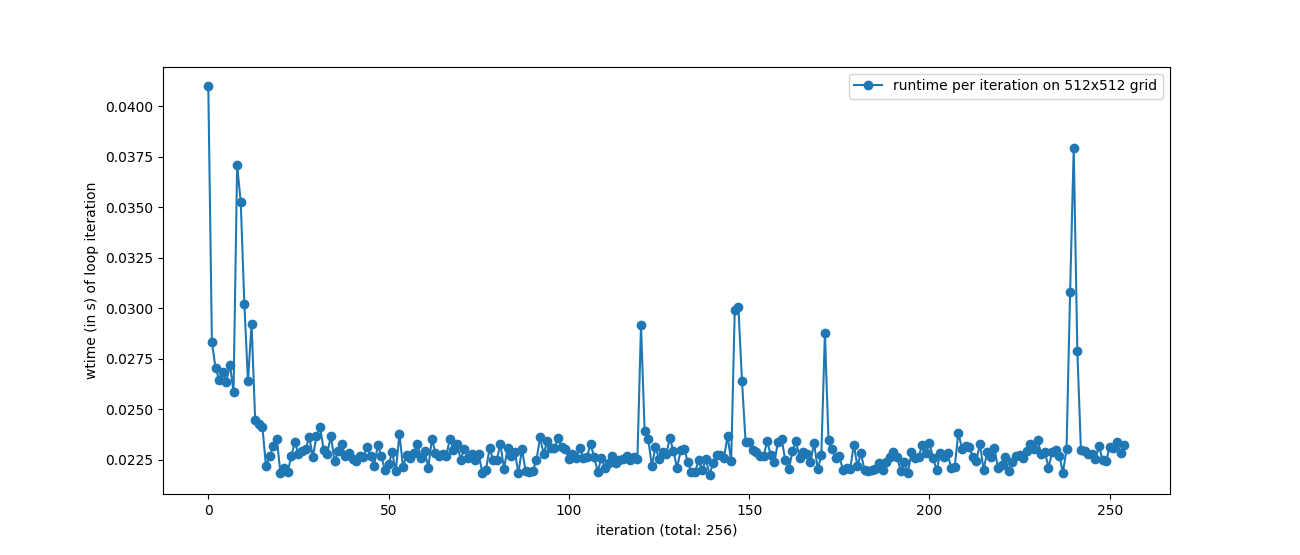
\includegraphics[width=0.9\textwidth]{imgs/runtime_baseline_per_iteration}
  \caption{Runtime per iteration on 2020 macbook air}
  \label{fig:runtime_per_iteration}
\end{figure}
Important to note is that the total number of timesteps computed increases by introducing finer grid sizes.
With other words, simulating two seconds using a fine grid uses more iterations than simulating two seconds using a corse grid. 
The reason is that $dt$ is computed each loop, which is dependent on $dx$, the granularity of the mesh.

The second important parameter is the grid size.
Finer grids allow for higher precision but increase the computational complexity quadratically.
To measure runtime over a variety of gridsizes, we decided to keep the number of time steps constant.
We simulated 256 timesteps over all grid sizes and performed each computation three times, which we then averaged.
\todo{Insert graphic of all baseline runs!}

\section{Optimizations using Cython}
\section{Optimizations using Pytorch}
The original implementation makes heavy use of numpy functionalities.
All data is stored as numpy arrays that are incrementally updated using the computed fluxes.
This provides an easy approach to move the computations on a GPU using pytorch.
Pytorch's computations are run using tensors --- an immutable datatype that shares resemblence with numpy arrays.
A big difference however is that tensor operations are supported to be computed using accelerators.
Due to the fact that pytorch mirrors numpys interface, we simply need to convert said numpy arrays to pytorch tensors
and tell pytorch to perform the computations using GPU compatible hardware.
\todo[inline]{insert figure of GPU runtimes}

To compare the performance on a wider range of grid sizes, we chose to limit the simulation to a fixed number time steps.
As one can see\todo{describe figure before referencing it} in the results of figure, making use of accelerators *greatly* improves the overall runtime for larger grid sizes.
As noted above \todo{insert ref to figure}, for finer grids this means we simulate less time in total.

\section{Optimizations using Dask}

\section{Conclusion}
\section{Appendix:}

% content end
%###############################################################################

% TODO: bibliograpghy when needed
% \printbibliography

\end{document}
